\documentclass[11pt]{article}
\usepackage[utf8]{inputenc}
\usepackage{hyperref, amsmath, amssymb, amsthm, graphicx, fancyvrb, enumitem, titlesec, setspace, float, fancyvrb, minted}
\usepackage[dvipsnames]{xcolor}
\usepackage[top=1in, bottom=1in, left=1.25in, right=1.25in]{geometry}

\titleformat{\section}{\normalfont\bfseries}{}{0em}{}
\titlespacing*{\section}{0pt}{1.5ex plus .2ex minus .2ex}{0.8ex plus .1ex}
\begin{document}
\noindent Andre Winkel, Russell Yang \hfill \today \\
\rule{\textwidth}{0.4pt}

\begin{center} \large {\textbf{Lab 1}} \\[0em] 
{EE115, Introduction to Communication Systems, Fall 2025} \end{center}

\section{Problem 1: Examining a random signal and AM power efficiency}
In this problem, we will examine the average power of a random signal that has
its minimum value larger than or equal to $-1$, and also examine its impact on the power
efficiency of conventional amplitude modulation (AM) signals.
\begin{enumerate}[label=\textbf{\alph*)}, leftmargin=2.6em]
    \item We begin by using the Gaussian-random-number generator to generate a random sequence
    \begin{equation} \notag
        m[1], m[2], \dots, m[N]
    \end{equation}
    where we will set $N$ as $200$ [a large integer].
    We can do so in MATLAB by employing the \texttt{randn} function.

    \item We can then use the \texttt{min} function in order to determine the 
    minimum value of our sequence, which we can denote by $-M_0$. Verbatim, 
    \verb|m_nk = 1/M_0 * m_k; min(m_nk);|.

    \item We can then compute the normalized sequence
    \begin{equation}
        m_n[k] = \frac{1}{M_0}m[k],
    \end{equation}
    where its minimum value is found to be
    \begin{equation} \notag
        m_n[k] = -1.
    \end{equation}

    \item We can then compute the average power with
    \begin{equation}
        P_m = \frac{1}{M} \sum_{k=1}^{N} m^2_n[k].
    \end{equation}
    In MATLAB, this is achieved with \verb|P_m = (1/N) * sum(m_nk.^2)|.

    \item Considering the power efficiency of the AM signal, we can determine
    its power efficiency through
    \begin{equation}
        \eta_{AM} = \frac{a_{mod} P_m}{1+a_{mod} P_m}.
    \end{equation}
    We can plot $\eta_{AM}$ versus $P_m$ subject to $0<P_m<1$ for each of 
    $a_{mod}=1, 0.75, 0.5$ in MATLAB, where we observe the following plot:
    \begin{figure} [H]
        \centering
        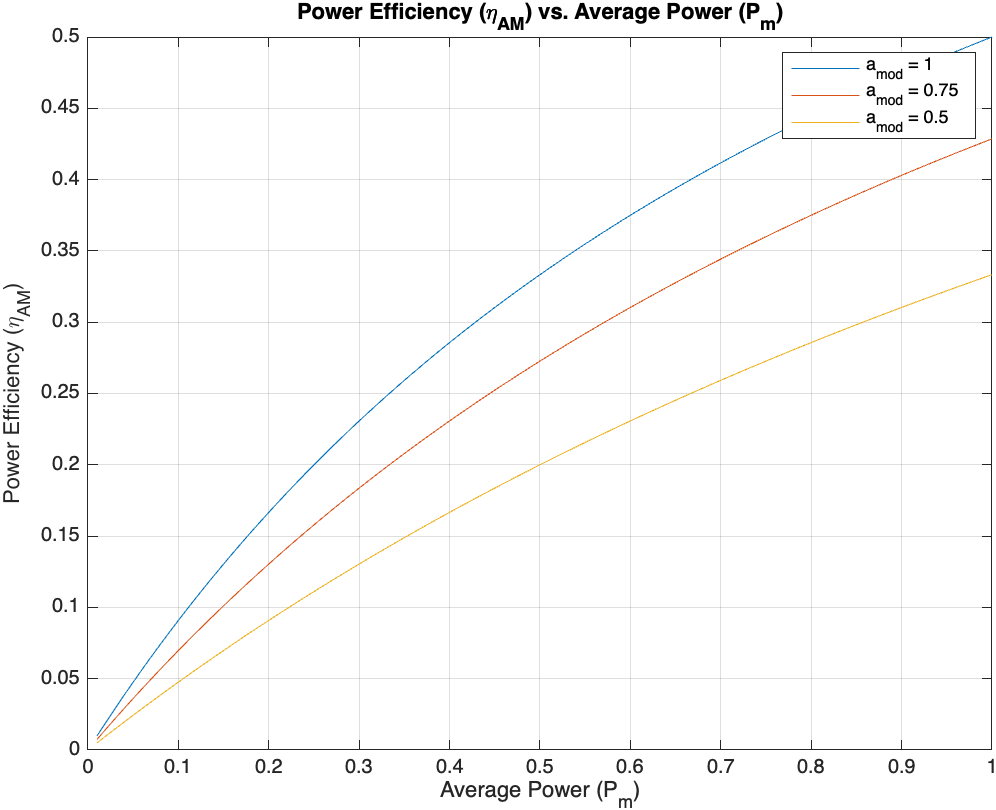
\includegraphics[width=0.6\linewidth]{plot1.png}
    \end{figure}

    \item Selecting some values of a random run of the MATLAB program thus frar,
    we observe $\eta_{AM}$ for each of $a_{mod}=1, 0.75, 0.5$ using
    the same $P_m$ as before. An example run allows us to obtain the values\\
    \begin{equation} \notag
        \eta_{AM} = 0.1682 : a_{mod} = 1
    \end{equation} 
    \begin{equation} \notag
        \eta_{AM} = 0.1317 : a_{mod} = 0.75
    \end{equation} 
    \begin{equation} \notag
        \eta_{AM} = 0.0918 : a_{mod} = 0.5
    \end{equation} 
    where it becomes evident, once interpreting the respective $\eta_{AM}$ values
    as percentages, that conventional amplitude modulation is a very power-inefficient
    method of transmission.

\end{enumerate}

\section{Problem 2: Examining the quality of a simple DC blocker}
In this problem, we will examine the quality of a simple DC blocker which consists
of a capacitor $C$ and a resistor $R$ in series. We are given the frequency response
of the DC blocker,
\begin{equation}
    H(f) = \frac{R}{R+\frac{1}{j2\pi C}} = \frac{j2\pi f}{j2\pi f + \frac{1}{RC}}.
\end{equation}

\begin{enumerate}[label=\textbf{\alph*)}, leftmargin=2.6em]
    \item Plotting $|H(f)|$ versus $f$ for $|f|<B$ for each of $RC=0.01,0.1,1,10$, we
    observe the following plots:
    \begin{figure} [H]
        \centering
        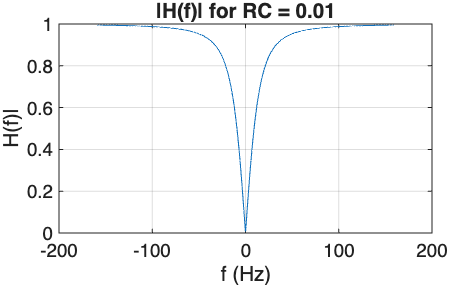
\includegraphics[width=0.4\linewidth]{plot2.png}
        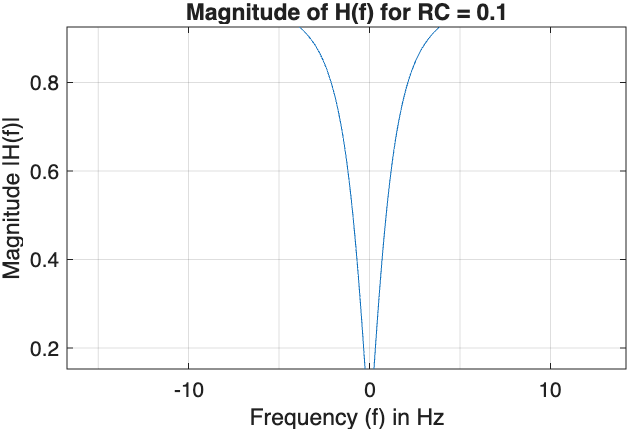
\includegraphics[width=0.4\linewidth]{plot3.png}
        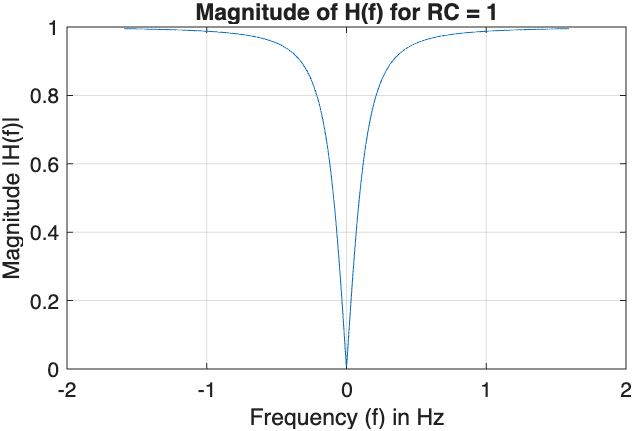
\includegraphics[width=0.4\linewidth]{plot4.png}
        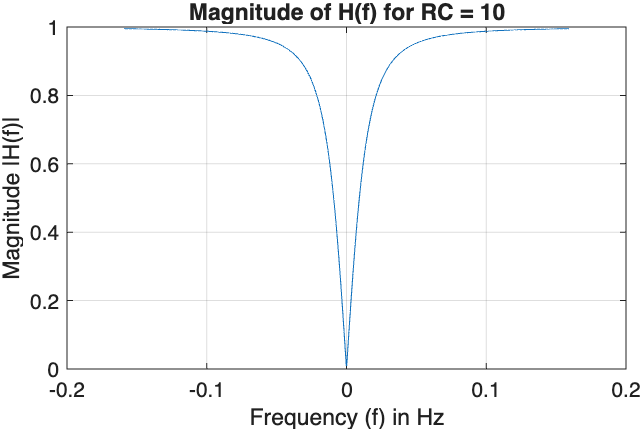
\includegraphics[width=0.4\linewidth]{plot5.png}
    \end{figure}
    Here, we chose $B$ such that $B=\frac{10}{2\pi RC}$ for each of the
    respective $RC$ values. This is an appropriate choice, as it allows us to
    observe the behavior of $|H(f)|$ as it approaches its asymptotic value
    of $1$. We are also able to observe the stopband behavior of the DC blocker
    as $f$ approaches $0$, and everything in between.

    \item We can then repeat the above but plotting $20\log_{10} |H(f)|$ versus $f$.
    Additionally, we set the vertical range to be from $-60\text{dB}$ to $0\text{dB}$. We observe the following plots:
    \begin{figure} [H]
        \centering
        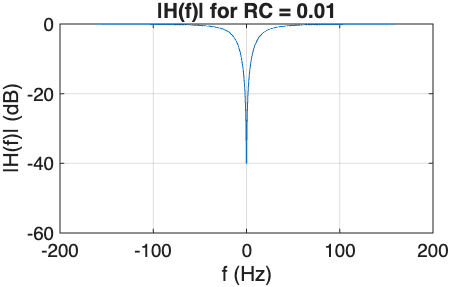
\includegraphics[width=0.4\linewidth]{plot6.png}
        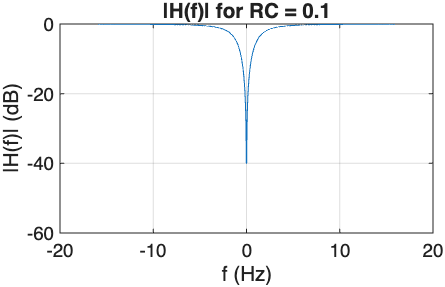
\includegraphics[width=0.4\linewidth]{plot7.png}
        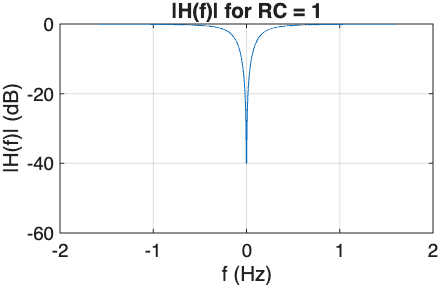
\includegraphics[width=0.4\linewidth]{plot8.png}
        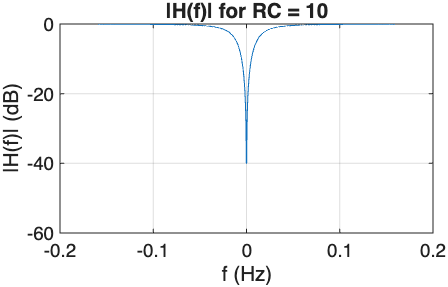
\includegraphics[width=0.4\linewidth]{plot9.png}
    \end{figure}
    and we observe that MATLAB dictates our filter to bottom out at $-40\text{dB}$. We
    also know that the ideal filter will have a gain of $-\infty\text{dB}$ at $f=0$.

    \item Considering our transfer function $H(f)$ and the requirement $0.95<=|H(f=20\text{Hz})<=1$, 
    we can find that
    \begin{equation} \notag
        \text{RC}_{\text{min}} = \sqrt{\frac{(\text{gain}_\text{min}=0.95)^2}{(2\pi f)^2 \cdot (1-(\text{gain}_\text{min}=0.95)^2)}}.
    \end{equation}
    Using MATLAB to solve, we determine
    \begin{equation} \notag
        \text{RC}_{\text{min}} \approx 0.0242.
    \end{equation}
\end{enumerate}

\end{document}